\documentclass{article}
\usepackage[dvipsnames]{xcolor}
\usepackage{tikz}
\usepackage{ifthen}
\usetikzlibrary{shapes.misc, shapes.geometric, decorations.pathreplacing, calc, patterns, external}
\tikzexternalize[prefix=figures/]
\tikzset{external/force remake}

% Define some colors
\definecolor{generic}{named}{ProcessBlue}
\definecolor{beam}{named}{ProcessBlue}
\definecolor{light}{named}{BurntOrange}
\definecolor{heavy}{named}{Rhodamine}
\definecolor{line}{named}{Plum}

% Declare objects
\tikzset{
  pics/track/.style args={#1/#2/#3/#4/#5/#6}{
      code = {
          \pgfmathsetmacro{\xbegin}{#1}
          \pgfmathsetmacro{\ybegin}{#2}
          \pgfmathsetmacro{\angle}{#3}
          \pgfmathsetmacro{\radius}{#4}
          \pgfmathsetmacro{\w}{0.3} % width in Y dim
          \pgfkeys{/track color/.initial=red}
          \ifthenelse{\equal{#5}{}}{%
          }{
            \pgfkeys{/track color=#5}
          }
          % Coordinates 
          \coordinate (begin) at (\xbegin, \ybegin);
          \coordinate (end) at (\xbegin + \radius, \ybegin);
          \coordinate (a) at (\xbegin, \ybegin - \w / 2);
          \coordinate (b) at (\xbegin, \ybegin + \w / 2);
          \coordinate (c) at (\xbegin + \radius, \ybegin + \w / 2);
          \coordinate (d) at (\xbegin + \radius, \ybegin - \w / 2);
          % Transform coordinates
          \coordinate (arot) at ($(begin)!1!\angle:(a)$);
          \coordinate (brot) at ($(begin)!1!\angle:(b)$);
          \coordinate (crot) at ($(begin)!1!\angle:(c)$);
          \coordinate (drot) at ($(begin)!1!\angle:(d)$);
          % Track
          \fill[fill=\pgfkeysvalueof{/track color}, rounded corners=0.75mm] (arot) -- (brot) -- (crot) -- (drot) --cycle;
          % Fit 
          \ifthenelse{\equal{#6}{}}{}{
            \draw[very thick,black] (begin) -- ($(begin)!1!\angle:(end)$);}
        }
    },
  pics/track/.default=0/3/0/3/green
}
\tikzset{
  pics/actar/.style args={#1}{
    code = {
        \useasboundingbox (-0.75, -0.75) rectangle (6.25, 6.25);
        % Coordinates for rectangle
        \coordinate (a) at (0,0);
        \coordinate (b) at (0,6);
        \coordinate (c) at (6,6);
        \coordinate (d) at (6,0);
        \draw[very thick, black, fill opacity=0] (a) -- (b) -- (c) -- (d) -- cycle;
        \node at ($(a)!0.8!(d)$) [below=0.05cm] {\Large X};
        \node at ($(a)!0.8!(b)$) [left=0.05cm] {\Large #1};
    }
  },
  pics/actar/.default=Y
}

\begin{document}
\section{Filter}
\subsection{BreakChi2}

Initial approach:

\tikzsetnextfilename{break_chi2_0}
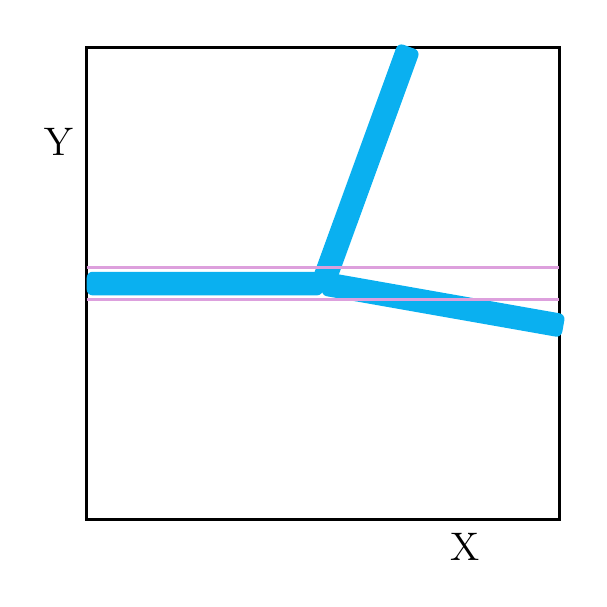
\begin{tikzpicture}
	\pic {actar};

	\pic (beam) {track={0/3/0/3/generic/}};
	\pic (light) {track={3/3/70/3.2/generic/}};
	\pic (heavy) {track={3/3/-10/3.1/generic/}};

	% define line coordinates
	\coordinate (up0) at (0, 3.2);
	\coordinate (up1) at (6, 3.2);
	\coordinate (low0) at (0, 2.8);
	\coordinate (low1) at (6, 2.8);
	\draw[very thick, line] (up0) -- (up1);
	\draw[very thick, line] (low0) -- (low1);
\end{tikzpicture}

After applying the breakchi2 operation:

\tikzsetnextfilename{break_chi2_1}
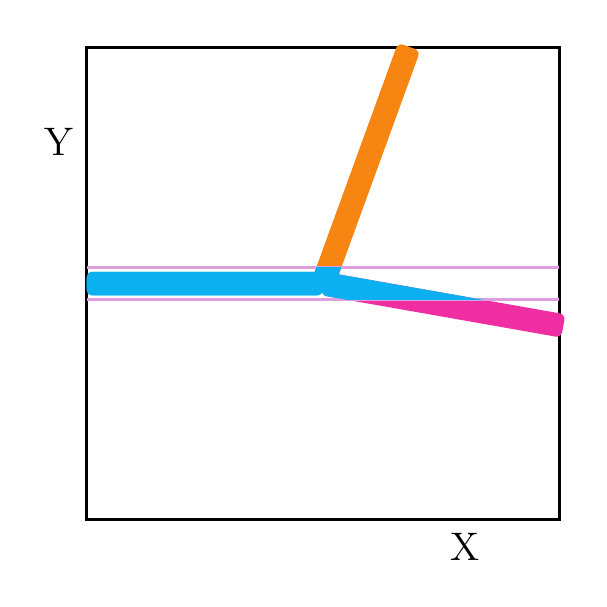
\begin{tikzpicture}
	\pic {actar};

	\pic (beam) {track={0/3/0/3/generic/}};
	\pic (light) {track={3/3/70/3.2/light/}};
	\pic (heavy) {track={3/3/-10/3.1/heavy/}};

	% define line coordinates
	\coordinate (up0) at (0, 3.2);
	\coordinate (up1) at (6, 3.2);
	\coordinate (low0) at (0, 2.8);
	\coordinate (low1) at (6, 2.8);
	\draw[very thick, line] (up0) -- (up1);
	\draw[very thick, line] (low0) -- (low1);

	\begin{scope}
		\clip (up0) -- (up1) -- (low1) -- (low0);  % Clip between the lines
		\pic (beam) {track={0/3/0/3/generic/}};
		\pic (light) {track={3/3/70/3.2/generic/}};
		\pic (heavy) {track={3/3/-10/3.1/generic/}};
	\end{scope}
\end{tikzpicture}

\subsection{Merge broken tracks}

\tikzsetnextfilename{merge}
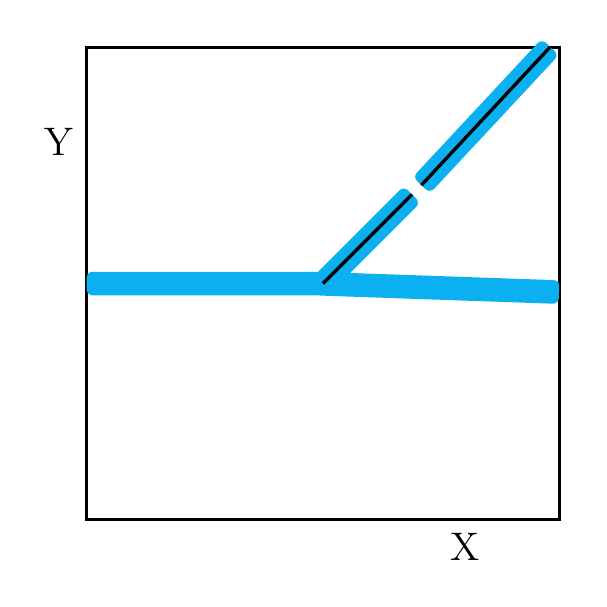
\begin{tikzpicture}
	\pic {actar};

	\pic (beam) {track={0/3/0/3/generic/}};
	\pic (heavy) {track={3-0.1/3/-2/3.1/generic/}};
	\pic (light) {track={3/3/45/1.6/generic/true}};
	\pic (light) {track={4.25/4.25/47/2.4/generic/true}};
\end{tikzpicture}

\subsection{Pileup}
\tikzsetnextfilename{pileup}
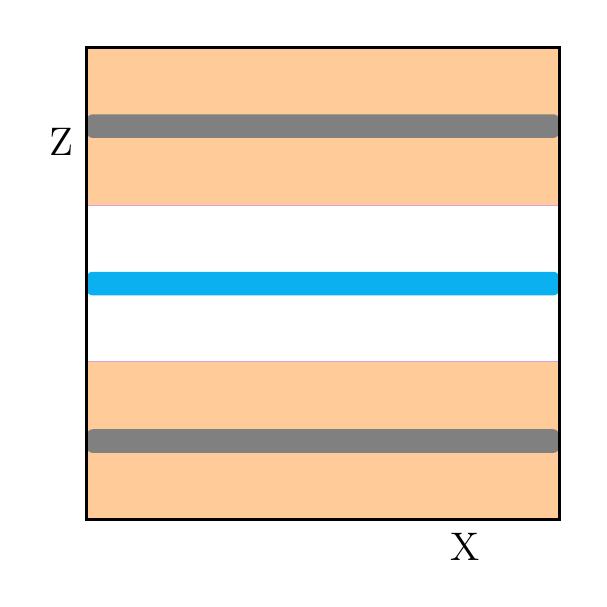
\begin{tikzpicture}

	% define line coordinates
	\coordinate (up0) at (0, 4);
	\coordinate (up1) at (6, 4);
	\coordinate (low0) at (0, 2);
	\coordinate (low1) at (6, 2);
	\draw[very thick, line] (up0) -- (up1);
	\fill[orange!40] (up0) -- (up1) -- (6,6) -- (0,6) -- cycle;
	\draw[very thick, line] (low0) -- (low1);
	\fill[orange!40] (low0) -- (low1) -- (6,0) -- (0,0) -- cycle;

	\pic (beam) {track={0/3/0/6/generic/}};
	\pic (other) {track={0/5/0/6/gray/}};
	\pic (other) {track={0/1/0/6/gray/}};

	\pic {actar={Z}};
\end{tikzpicture}

\subsection{Fine analysis of tracks}
It's going to be difficult to get the same images as Juan has


\end{document}
